\documentclass{article}
\usepackage[utf8]{inputenc}
\usepackage{graphicx}

% comment about something
\author{Mikael Grön (473488), Anssi Moisio (),
    Visa Koski (), Lassi Knuuttila ()}
\title{Q-learning Project Plan - C++ ELEC-A7150}
\date{\today}

\begin{document}

\maketitle


\section{Q-learning}
In Q-learning the algorithm is simple, but when running it multiple times over
all the possible states, with all possible actions, the algorith can find the
optimal behavior of the system. The system consists of an actor that has a state
from which the actor can do some actions, that move the actor into a new state.
After every action the system gives the actor a revard (a punishment is a
negative revard). The optimal behavior is determined by how the revard is
maximized.


\subsection{Q-values}
Every compination of states and actions has a Q-value. These Q-values are
initialized all as 0. The optimal action in a state is the action with the
highest Q-value. When the system is learning, an action is performed, and the
Q-learning function updates the Q-value which is assosiated with the current
state and performed action:

\[Q(s_t, a_t) = Q(s_t, a_t) + \alpha [ r_t + \gamma \cdot max_aQ(s_{t+1}, a)
- Q(s_t, a_t) ]\]

Here $s_t$ is the current state, $a_t$ the current action,
$\alpha$ is the learning rate, $r_t$ is the revard from doing the action,
$\gamma$ is the discount factor, $max_aQ(s_{t+1}, a)$ is the next states
highest possible Q-value.

The Q-learning function makes the Q-values more accurate by testing out
the combinations of states and actions in the system. The Q-learning is an
optimisation method, which will find a optimal path, which gives the maximum
revard. The best path is the global maximum, but there can exist local maximums.
The local maximums can be avoided by introducing random actions in the learning
process. If the Q-learning has found a local maximum a random action will
hopefully try out someting that moves to the global maximum.

Teoretically the exact Q-values are found by running the learning process
for an infinitially long time. This is not practical (duh), so approximate
Q-values are enough. The learning needs to be terminated from outside, when an
satisfactory accuracy is achived.

To get accurate Q-values, the different combinations of states and actions
need to be tested multiple times during the learning process.
The number of Q-values are the number of states times the number of actions
in every state. Having a smaller amount of Q-values leads to a shorter learning
time. More Q-values can lead to more complex behavior for the learned actor.
This depends on the system.


\subsection{Modelling of Agents}
We model agents as a combination of sensors and actors. The sensors determine
which state the agent is in, and the actors can permorm actions.
We limit our systems to be two dimensional (2D), meaning the world and agents
are 2D. We will implement our program to support other 2D systems, but we
will start by studying a simple case of the agent in the picture:

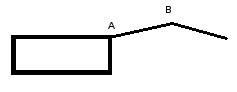
\includegraphics[width=0.8\textwidth]{simple_agent}

We will model this agent that moves trough a flat 2D world.
The agent gets a positive revard when it moves to the right, and a negative
revard when it moves to the left.

The agent has a body and an arm. The arm consists of two beams and two joints
(A and B). The joints angles determine the state of the actor, and actions are
performed by roteting the beams, changing the joints angles.
Both joints can move 360$^\circ$ continously, but we need to quantisize
the angles, so we can have a limited amount of states. We can also be wise
gods and limit the angle the joints can move. We can see that in our agents
case that the arm will not effect the state if it flails in the air, not
touching the ground. Also we say that the beam between the joints can not
occupy the same space as the body. Therefore we can limit the joints
permitted angles.

We limit the A joint to move 135$^\circ$, and the B joint to move
270$^\circ$. We quantisize the A joints angle into $2^4$ steps, and
the B joints angle into $2^5$ steps. This gives the actor
$2^4 \cdot 2^5 =$ \textbf{512 states}. The smallest angle registered at
the joint, due to the quantization, is
$135^\circ / 2^4 = 270^\circ / 2^5 \approx 8.4^\circ$.
The angle can be more precise, when simulating the agent, but the
Q-learning algorith will just "see" the quantizised angle.

A joint can be moved, by performing an action. We limit the movement to be
just one speed, which is one quantization step. A joint can only move
clockwise, counterclockwise or not move at all. Multiple joints rises the
possible actions to be 3 to the power of the number of joints. Our
agent has two joints, therefore there is $3^2$ = \textbf{9 actions} to
perform in a state.

The number of Q-values is states times actions. Therefore there is
$512 \cdot 9$ = \textbf{4608 Q-values}. This should be a manageable
amount to use the Q-learing algorithm on. If a Q-value is a float,
wich is 4 bytes, then the Q-values will occupy 18KB of memory.
Thus the memory size would be tolerable, even when having multiple agents
at the same time learning.


\section{Class Structure}
The main divide of the program is; the learning and the simulation. The
simulation and the learning parts communicate with eachother mainly by the
learning part telling the simulation to do an action. The simulation will then
simulate the action, returning the new simulated change of the agent, to the
learning part. The learning part evaluates the simulated change, determining
what the revard for the performed action was, updating the Q-value.
And so on.

\textbf{Insert here the UML picture.}


\subsection{Agent}
The spesifications of the agent contain; actors, sensors, physical form.


\subsection{Q-learning}
Anssi is a creative boy, and hopfully will find something to say about this
divide...

Q-Value-table; revardFunction; Q-function; doRandomActionFunction


\subsection{Simulation}
The simulation is divided into the graphics and the physics...bla bla blaa...


% Parts under this line will not exist in the final version. 
\newpage

\section{Using Latex}
Compile to pdf with command: \textbf{pdflatex plan.tex}

The pdf can be read with okular.
The open file is updated in the reader, when again compiling.

\end{document}
